\section{Implementation}\label{sec-implementation}

We implemented the prototype on Linux/x86 arch. Specifically, we implemented the code generator with LLVM 9.0.0, and built other parts on an SGX environment.
The LLVM passes consist of several types of instrumentations for the code generator. 
Besides, we implemented the bootstrap enclave based on Capstone~\cite{capstone} as the disassembler. 

%from scratch and made a best effort to reduce the size of the trusted computing base, where consists of about 1900 lines of code in total.
%Yet the loader we implemented is very small that only consists of less than 400 lines of C code, while the verifier consists of less than 500 lines that is made from scratch.

%\wenhao{stack guard page}\weijie{add it in the following subsection}

%\subsection{Assembly-level Instrumentation}\label{subsec-instrument}
\subsection{Multi-level Instrumentation}\label{subsec-instrument}

%\xiaofeng{To support flexible control of code to comply with different security policies, we implanted a set of switches into our code generator. These switches work on the IR level and their on/off states can be passed down to the target code level for further control, depending on the policies to be enforced. In this way, we separate  This \textit{separating mechanism and policy} design and implementation can make our frame more scalable and flexible for various security policies. }


\begin{figure}[htbp]
\centerline{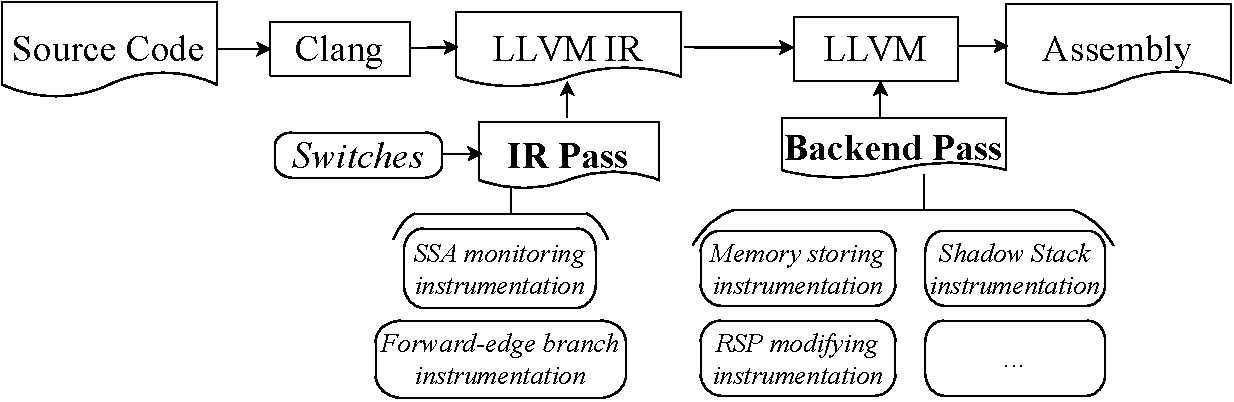
\includegraphics[scale=0.42]{figures/fg-codegen.pdf}}
\caption{ Workflow of flexible code generation}\label{fg-codegen}
%\wenhao{please update Hyperrace to SSA monitoring}
\vspace{-8pt}
\end{figure}

The code generator we built is mainly based on LLVM (Fig.~\ref{fg-codegen}), and the assembly-level instrumentation is the core module. 
More specifically, we implemented modules for checking memory writing instructions, RSP modification, indirect branches and for building shadow stack. We also reformed an instrumentation module to generate side-channel-resilient annotations. 
To support flexible control of different security policies, we implanted a set of switches into our code generator. These switches work on the IR level and their on/off states can be passed down to the target code level for further control, depending on the policies to be enforced. On the in-enclave verifier side, we also use this \textit{separating mechanism and policy} design, allowing for smooth integration of a loading-time pass that supports a new mitigation scheme. More specifically, we provide high-level APIs that allows the developers to implement their instrumentation and validation passes and plug them into the loader~\cite{our-prototype}.
 

Here is an example (Figure~\ref{fg-mov}). The main function of the module for checking explicit memory write instructions (P1) is to insert annotations before them. Suppose there is such a memory write instruction in the target program, `\texttt{mov reg, [reg+imm]}',
the structured annotation first sets the upper and lower bounds as two temporary Imms (0x3ffffffffffff and 0x4ffffffffffff), and then compares the address of the destination operand with the bounds. The real upper/lower bounds of the memory write instruction are specified by the loader later. If our instrumentation finds the memory write instruction trying to write data to illegal space, it will cause the program to exit at runtime. 
%\revise{The code snippet (structured format of the annotation) is shown in Figure~\ref{fg-mov}.}

%\weijie{more explanation here with Hoare logic}


%\revise{The code snippet (structured format of the annotation) is shown in Figure~\ref{fg-mov}. 
%\weijie{more explanation here with Hoare logic}}
%More details can be found at Appendix~\ref{appendix-instrumentation}.

\begin{figure}
\begin{center}
\begin{minipage}{0.4\textwidth}
%[basicstyle=\scriptsize,numbers=left, numberstyle=\scriptsize,,keywordstyle=\color{blue!70},commentstyle=\color{red!50!green!50!blue!50}, rulesepcolor=\color{red!20!green!20!blue!20}]
\begin{lstlisting}[basicstyle=\scriptsize]
pushq   %rbx    ;save execution status
pushq   %rax
leaq    [reg+imm], %rax ;load the operand
movq    $0x3FFFFFFFFFFFFFFF, %rbx  ;set bounds
cmpq    %rbx, %rax
ja      exit_label
movq    $0x4FFFFFFFFFFFFFFF, %rbx  ;set bounds
cmpq    %rbx, %rax              
jb      exit_label
popq    %rax
popq    %rbx
movq    reg, [reg+imm]
\end{lstlisting}
\end{minipage}
\end{center}
\vspace{-8pt}
\caption{Store instruction instrumentation}\label{fg-mov}
\vspace{-15pt}
\end{figure}

%Although using the code generator we could automatically produce an instrumented object file, we still need to deal with some issues manually that may affect practical usage. As the workflow described in Figure~\ref{fg-workflow}, the first job to make use of CAT system is preparing the target binary.  Service-specific libraries and some dependencies also should be built and linked against the target program (detailed in Appendix~\ref{appendix-preparing}).
%Nevertheless, we have to do some preparing work before the target program loading~\ref{appendix-preparing}.

\subsection{Building Bootstrap Enclave}\label{subsec:bootstrap-impl}
%\begin{figure}[htbp]
\centerline{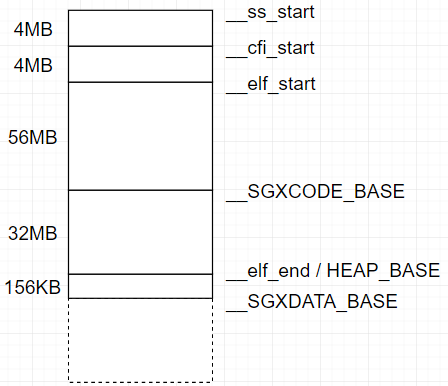
\includegraphics[scale=0.42]{figures/memlayout.png}}
\caption{Memory Layout}\label{fg-memlayout}
\label{fig}
\end{figure}
%\vspace{3pt}\noindent\textbf{Reserving Blank Memory Space.}
Following the design in Section~\ref{subsec:verify}, we implemented a \textit{Dynamic Loading after RA mechanism} for the bootstrap enclave. The enclave is initiated based upon a configuration file (a.k.a. the manifest file), which specifies the system calls the enclave is allowed to make in compliance with security policies, the protection enforced through instrumented OCall stubs. During the whole service, the data owner can only see the attestation messages related to the bootstrap's enclave quote, but learn nothing about service provider’s code.

%\xiaofeng{Just like Graphene-SGX~\cite{} and Occlum~\cite{}, our approach necessary OCalls for enforcing P0 can be prescribed with a configuration file.}

\begin{figure}[htbp]
\centerline{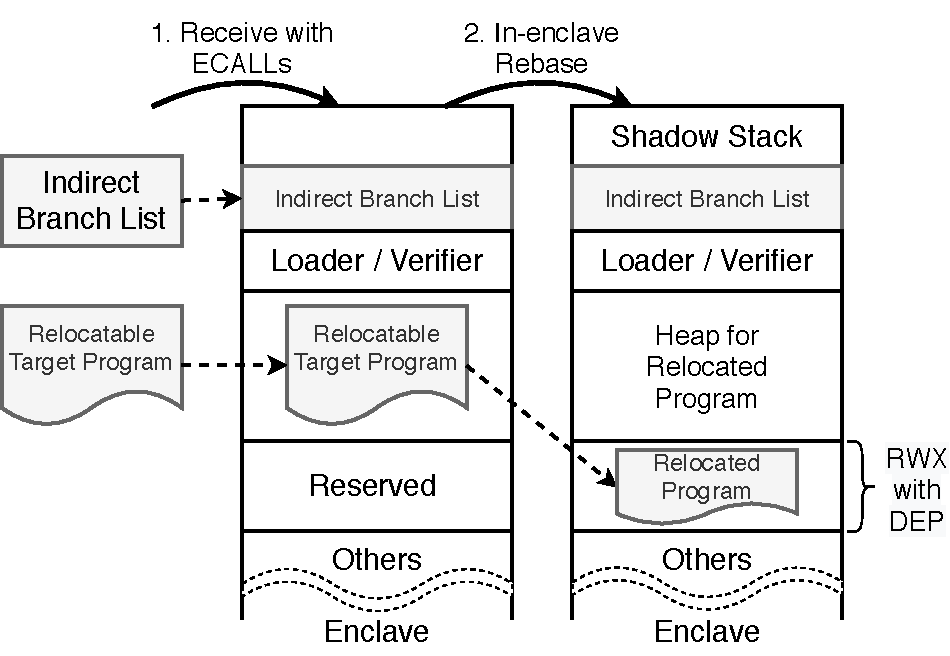
\includegraphics[scale=0.45]{figures/fg-dynloader.pdf}}
\caption{Detailed workflow of the dynamic loader}\label{fg-dynloader}
\vspace{-10pt}
\end{figure}

\vspace{3pt}\noindent\textbf{Remote attestation}.\label{subsec:ra-impl}
Once the bootstrap enclave is initiated, it needs to be attested. 
\revise{We leverage the RA-TLS routine}~\cite{knauth2018integrating} and adjust it to our implementation.
The conception of “Role” (code owner or data owner) is incorporated in RA-TLS, to make sure the bootstrap enclave can distinguish the two parties and communicate with them using different schemes.
%We leverage the original RA routine~\cite{originalra} and adjust it to our design. 
%The original RA routine requires that the host, which is assumed to run the enclave as the `client', initiates the attestation towards the `server', who owns the data. While in this CCaaS scenario, the service runs in the enclave while the remote user owns the data. So, we modify this routine to enable a remote CCaaS user to initiate the attestation.
The RA procedures are invoked inside the bootstrap enclave after secret provision between parties. After obtaining a quote of the bootstrap enclave, the remote data owner submits the quote to IAS and obtains an attestation report. 
%This report is signed by the IAS report signing private key, which can be validated by the data owner.

%\xinyu{I think the following paragraph is slightly misleading because in my implementation, RA is actually initiated by the remote user. The reason why RA should be invoked by user is stated in the first paragraph of the Remote Attestation part.}
%Using our customized Remote Attestation flow, service provider’s enclave can be attested right after enclave initialization. Since the loader/verifier code is public, the RA procedures can be invoked by simply calling \verb|sgx_ra_init()| inside the service provider’s enclave after secret provision between the remote user and the service provider. After obtaining an enclave quote of the current running enclave which is signed with the platform's EPID key, the remote data owner can submit the quote to IAS and obtain an attestation report. This report is signed by the IAS Report Signing private key, and the remote user can validate this signature using the IAS Report Signing Public Key.


\vspace{3pt}\noindent\textbf{Dynamic loader}. 
When the RA is finished, trust between the data owner and the bootstrap enclave is established. The user then can locally/remotely call Ecall (\verb|ecall_receive_binary|) to load the service binary instrumented with security annotations and the indirect branch list without knowing the code. 
User data is loaded from untrusted memory into the trusted enclave memory when the user remotely calls Ecall (\verb|ecall_receive_userdata|), to copy the data to the section reserved for it.

% \revise{Just like Graphene-SGX~\cite{} and Occlum~\cite{}, necessary OCalls for enforcing P0 can be prescribed with a configuration file.}

Then, the dynamic loader in the bootstrap enclave loads and relocates the generated code. 
The indirect branch list, which is comprised of symbol names that will be checked in indirect branch instrumentations, will be resolved at the very beginning. 
%Those symbol names will be replaced with the value of addresses, i.e., their actual addresses in the enclave memory space. %\xinyu{actually in our implementation, ECALL ecall\_receive\_entrylabel is first called before ecall\_receive\_binary} %The dynamic loading procedure is invoked when the user remotely calls ECALL (\verb|ecall_receive_entrylabel|). 
The memory size of our bootstrap enclave when initialing is about 96 MB by default, including 1 MB reserved for shadow stack, 1 MB for indirect branch targets, 64 MB for data, 28 MB for service binary code, and less than 2 MB of the loader/verifier.
After loading the service binary, the memory cost would be the size of the service binary plus the necessary libraries (e.g., libc, mbedtls, etc.).



%\revise{And we reserve more than 32M memory space for received binary and for `.data' section, which also can be configured in the manifest file.}

\vspace{3pt}\noindent\textbf{Policy verifier}.\label{subsec-boundarychecking}
The policy-compliance verifier, is composed of three components - a clipped disassembler, a verifier, and an immediate operand rewriter.

\vspace{2pt}\noindent$\bullet$\textit{ Clipped disassembler.} 
We enforce each policy at assembly level. 
Thus, we incorporate a lightweight disassembler inside the enclave. To implement it, we remove unused components of this existing wide-used framework, and use Recursive Descent Disassembly to traverse the code. When dealing with conditional branching instructions, we add call/jump target instructions to a list of deferred code to be disassembled at later time using the recursive descent algorithm. As a control flow-based algorithm, it can provide very complete code coverage with minimal code.
Also, we use the \textit{diet} mode, making the engine size at least 40\% smaller~\cite{quynh2014capstone}. The clipped Capstone consists of 9.1 KLoC as the base of our verifier.



\vspace{2pt}\noindent$\bullet$\textit{ Policy verifier.}\label{subsec-policyverifer}
The verifier and the following rewriter do the work just right after the target binary is disassembled, according the structured guard formats provided by our code generator. The verifier uses a simple scanning algorithm to ensure that the policies are applied in assembly language instrumentation. 
%Then, the verifier's job is done and the proof (instrumentations) will do the magic - checking policies. 
Specifically, the verifier scans the whole assembly recursively along with the disassembler. It follows the clipped disassembler to scan instrumentations before/after certain instructions are in place, and checks if there is any branch target pointing between instructions in those instrumentations.
%Moreover, legal jump addresses can be obtained from symbol tables by searching indirect branch target names.

\vspace{2pt}\noindent$\bullet$\textit{ Imm rewriter.}\label{subsec:immrewriter} One last but not least step before executing the target binary code is to resolve and replace the Imm operands in instrumentations, including the base of the shadow stack, and the addresses of indirect branch targets (i.e. legal jump addresses). For example, the genuine base address of shadow stack is the start address \verb|__ss_start| of the memory space reserved by the bootstrap enclave for the shadow stack. The ranges are determined using functions of Intel SGX SDK during dynamic loading (Section~\ref{subsec:verify}).
%With unknown addresses replaced to corresponding addresses in the enclave memory (by the Imm rewriter in Subsec.~\ref{subsec:immrewriter}), the binary code is prepared for privacy policy compliance verification.
%We use the simplest way to rewrite Imm operands.

